\subsection{Thrust 2: Scalable Runtime Trust Attestation.}
\label{sb:t2}

\textbf{Problem Statement.}
Establishing a trusted execution domain, or simply bootstrapping firmware in the Normal world, does not guarantee that it continues to execute as intended.
Secure boot and conventional remote attestation establish only properties of the loaded software or the initial system state, leaving runtime control-flow hijacking attacks undetected.
An attacker who exploits a runtime vulnerability can therefore redirect control flow (e.g., ROP, JOP exploits), manipulate task execution, or abuse asynchronous system events without changing the initially attested binary.
Control-flow attestation (CFA) addresses part of this problem by allowing a remote verifier to reason about the execution path taken by a program.
However, existing CFA approaches are difficult to apply to realistic embedded systems because their evidence or measurement cost may grow with execution duration or program complexity, while protected-domain transitions and cryptographic operations can introduce significant runtime overhead.

Embedded execution also differs fundamentally from the simple single-threaded program model assumed by many attestation schemes.
Bare-metal firmware and RTOS systems are event-driven and may include interrupts, exception handlers, callbacks, task scheduling, context switches, and interactions among privileged and unprivileged components.
These events alter the authorized execution state and can interleave with application control flow, making a conventional single-program trace insufficient.
Furthermore, the measurement state itself must remain protected while these asynchronous transitions take place.

This thrust therefore asks the following fundamental question:
\textbf{\textit{How can resource-constrained embedded systems generate compact and protected runtime evidence that enables a remote verifier to reason about authorized execution across long-running, interrupt-driven, and multitasking workloads without evidence growing with execution duration?}}
Addressing this requires new representations of execution, hardware-assisted measurement mechanisms, and verifier algorithms that capture
control-flow, task, interrupt, and other security-relevant events while bounding runtime, memory, and communication overhead.


\textbf{Related Work.}
Early remote attestation established only static software integrity or trustworthy execution state~\cite{seshadri2005pioneer,li2011viper,kong2014pufatt,armknecht2013security,eldefrawy2012smart}, not runtime control-flow hijacking.
Control-flow attestation (CFA) addresses this limitation by reporting execution behavior.
C-FLAT~\cite{abera2016c}, OAT~\cite{sun2020oat}, Blast~\cite{yadav2023whole}, DIAT~\cite{abera2019diat}, ARI~\cite{wangari}, ReCFA~\cite{zhang2021recfa}, SpecCFA~\cite{caulfield2024speccfa}, and ScaRR~\cite{toffalini2019scarr} explore different tradeoffs in trace granularity, evidence size, and verifier complexity, while CFA+~\cite{299850} combines local control-flow enforcement with lightweight attestation.
Specialized-hardware approaches, including VRASED~\cite{nunes2019vrased}, ACFA~\cite{caulfield2023acfa}, LiteHAX~\cite{dessouky2018litehax}, Tiny-CFA~\cite{nunes2021tiny}, LO-FAT~\cite{dessouky2017fat}, and IDA~\cite{arkannezhadida}, provide stronger monitoring capabilities but often rely on dedicated or modified hardware~\cite{neto2025pearts}.
Despite these advances, prior works are limited in supporting long-running, interrupt-driven, and multitasking execution while simultaneously bounding evidence size, runtime overhead, and verifier complexity.
Thrust~2 addresses this gap by developing scalable runtime evidence and verification mechanisms for realistic bare-metal and RTOS-based embedded systems.

\begin{wraptable}{r}{0.52\textwidth}
	\centering
	\vspace{-8pt}
	\footnotesize
	\setlength{\tabcolsep}{3pt}
	\begin{tabular}{lcccc}
		\toprule
		Scheme & Trace & Meas. & Verif. & Eval.\ size \\
		\midrule
		Naive trace & $O(l)$ & $O(1)$ & $O(l)$ & n/a \\
		OAT~\cite{sun2020oat} & $O(n)$ & $O(1)$ & $O(l|E|)$ & $n{<}1{,}000$ \\
		C-FLAT~\cite{abera2016c} & n/a & $O(2^{|V|})$ & $O(2^{|V|})$ & $|E|{=}322$ \\
		LO-FAT~\cite{dessouky2017fat} & n/a & $O(2^{|V|})$ & $O(2^{|V|})$ & $|E|{=}322$ \\
		Blast~\cite{yadav2023whole} & $O(2^{|V|})$ & $O(1)$ & $O(2^{|V|})$ & $|V|{<}987$ \\
		\textbf{\enola}~\cite{armanuzzaman2026enola} & $\mathbf{O(|V|)}$ & $O(1)$ & $O(2^{|V|})$ & $\mathbf{|V|{<}5{,}480}$ \\
		\bottomrule
	\end{tabular}
	\caption{\textit{Thurst2} foundation:Trace/measurement/verification complexity and largest evaluated size ($l$: executed branches, $n$: forward branches, $E$: CFG edges, $V$: basic blocks). \enola is the only scheme linear in program size.}
	\label{tab:enola}
	\vspace{-8pt}
\end{wraptable}

\textbf{Task 2.1: Compact and Verifier-Efficient Runtime Evidence}
We will investigate runtime attestation mechanisms that keep transmitted evidence, verifier cost, and prover-side runtime overhead practical as embedded applications grow larger, run longer, and move from bare-metal execution to a single task hosted on an RTOS.
Rather than recording complete execution traces whose size grows with the number of executed control-flow transfers, we will develop compact execution representations whose size is primarily determined by program basic blocks.
A central objective is to reduce this prover-side cost without weakening the integrity guarantees the verifier relies on.


As preliminary work, we developed \enola~\cite{armanuzzaman2026enola}: unlike prior approaches evaluated on multi-core Cortex-A processors or requiring hardware modifications, \enola targets a single-core, off-the-shelf Cortex-M85 ARMv8.1-M MCU, demonstrating that scalable control-flow evidence can be generated on commodity, resource-constrained embedded processors.
The verifier first sends a challenge, after which the TEE-hosted \enola attestation engine initializes the measurement keys and protection mechanisms.
During program execution, compiler-inserted instrumentation records a basic-block occurrence trace while ARM Pointer Authentication instructions incrementally compute separate measurements for forward and backward control-flow transfers.
The occurrence trace is maintained in TrustZone-protected memory, whereas the forward and backward measurements are retained in compiler-reserved registers so that neither is exposed in memory dumps.
At the end of execution, the collected evidence is combined with the verifier's challenge into an authenticated report and transmitted to the verifier, which reconstructs candidate execution paths and validates them against the received measurements.
This design makes the transmitted authenticator linear in the number of program basic blocks rather than the length of the executed path, substantially reducing communication cost relative to prior schemes (Table~\ref{tab:enola}).

\begin{comment}
% --- Original Task 2.1 "later" contribution (ambiguity-aware evidence for
% verifier-side path disambiguation), replaced with the store-hardening /
% TEE-overhead direction below per PI request -- kept here for reference. ---
Although \enola significantly reduces transmitted evidence, this compression exposes a new scalability challenge at the verifier.
Different execution paths can sometimes produce the same basic-block occurrence information, requiring the verifier to explore multiple candidate paths before finding one consistent with the received measurements.
This ambiguity can cause verification cost to grow rapidly for programs with increasingly complex control-flow structures.

Building on this observation, we will develop ambiguity-aware runtime evidence that introduces additional information only for portions of the control-flow graph where the compact representation is insufficient to uniquely characterize execution.
We will design static analyses to identify such ambiguous regions, determine what additional runtime information is necessary to distinguish their feasible paths, and generate this information selectively rather than increasing evidence for the entire program.
We will correspondingly develop verifier algorithms that use these localized hints to prune infeasible paths early and bound reconstruction effort around the ambiguous regions.
For continuously executing firmware, we will further investigate checkpointed and epoch-based attestation that periodically finalizes and authenticates bounded execution intervals, allowing runtime verification to continue indefinitely without requiring program termination or evidence growth proportional to total execution time.
\end{comment}

\enola's remaining bottleneck is not evidence size but how often it invokes TrustZone: eliminating backward-edge context switches still leaves forward-edge occurrence recorded through a trampoline call into the Secure world; our own evaluation attributes roughly a quarter of \enola's runtime overhead to these context switches.
We will extend \enola to a single task hosted on an RTOS by relocating occurrence-trace into an MPU-protected region of Normal-world memory, using \emph{store hardening}: Cortex-m's unprivileged store instructions check unprivileged-mode MPU permissions regardless of the processor's current privilege level, so a region can be made writable only by trace-recording instrumentation and unreachable from ordinary application, RTOS, or ISR code, avoiding a privileged-mode or Secure-world transition on every branch.
This replaces trust in TrustZone with a compiler-verified isolation property enforced by the MPU, so the guarantee holds even though the RTOS kernel itself remains outside the TCB, consistent with the threat model.
We will extend \enola's code scanner to also verify this MPU property and the forward-edge CFI check store hardening depends on.


\textbf{Task 2.2: Attestation of Interrupt-Driven and Multitasking Execution.}
Embedded systems rarely execute as a single linear control-flow path.
In RTOS-based firmware, hardware interrupts, timer-driven preemption, exception handling, and scheduler-mediated task switching create dynamic execution patterns that do not map cleanly to a single static control-flow graph.
As a result, attesting only the main application is insufficient: it cannot establish whether asynchronous and multitasking execution remained authorized, nor whether privileged transitions preserved the intended runtime trust boundary.
This task addresses the limitations of single-stream control-flow evidence by developing authenticated evidence for multiple execution contexts, including application tasks and interrupt handlers (Figure~\ref{fig:thurst22}).

\begin{wrapfigure}{r}{0.48\textwidth}
	\centering
	\vspace{-8pt}
	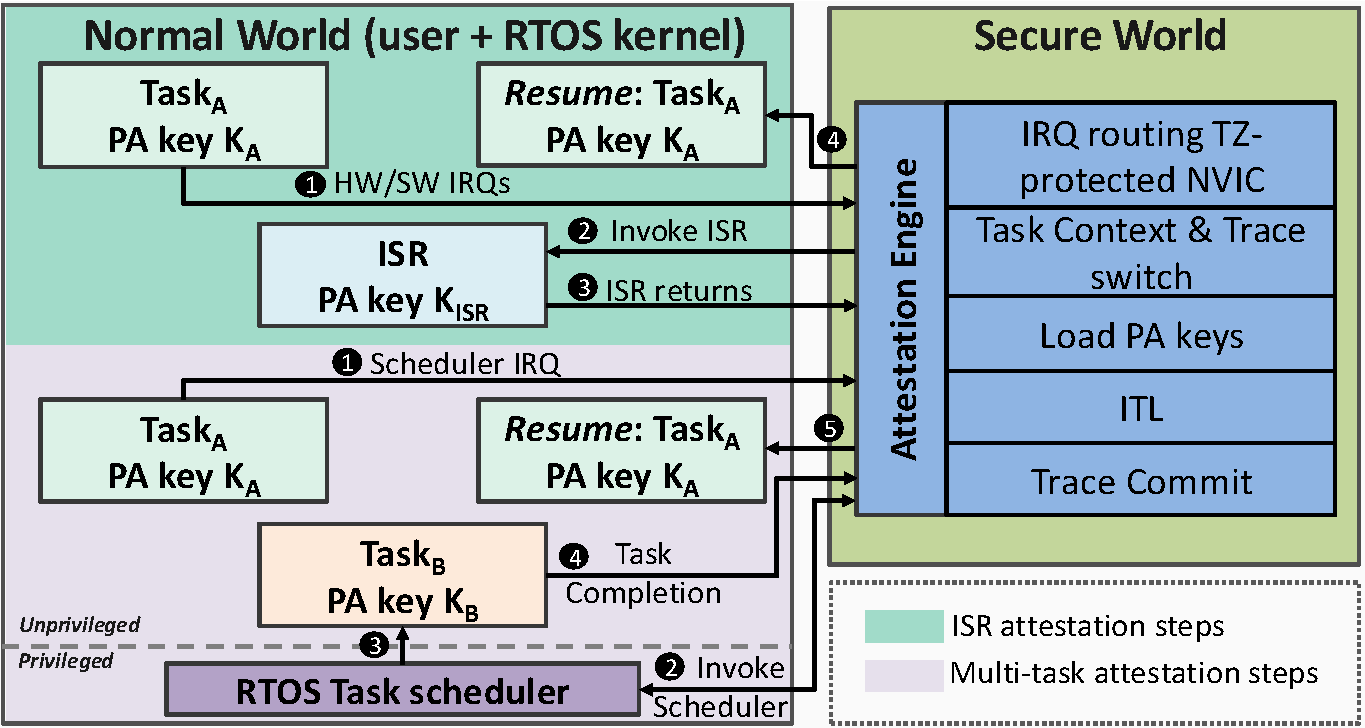
\includegraphics[width=0.46\textwidth]{figs/thrust2.2-rtos-attestation.pdf}
	\caption{Attestation framework for multitask and asynchronous-interrupt handling.}
	\label{fig:thurst22}
	\vspace{-10pt}
\end{wrapfigure}

A central challenge is to protect multiple concurrent measurement states and key bindings, i.e., one per task and ISR, without introducing excessive trusted-world transitions, memory overhead, or replay opportunities across context switches.

Based on the \enola attestation engine~\cite{armanuzzaman2026enola} and its Task~2.1 extension, we will develop a framework that addresses \enola's limitations of interrupt and multitask support, reusing the compiler instrumentation and PA-based measurement strategy described above for each individual execution context.
We will generalize this by assigning each task and ISR its own control-flow representation and per-context occurrence trace, recorded in the MPU-protected, store-hardened region from Task~2.1 rather than through a TrustZone call on every branch.
The interrupt controller and vector table are configured such that interrupts are routed to a transition handler before control reaches the scheduler or the ISR itself (Figure~\ref{fig:thurst22}).
This handler saves the currently active task's execution state and measurement context to the protected region, identifies the interrupt source and the next runnable context.
Because a task's PA key must stay confidential rather than merely tamper-evident -- a guarantee store hardening alone does not provide; thus key switching still crosses into TrustZone.
Before restoring the next task's CPU state, the scheduler triggers a secure call that loads the corresponding key or key slot from a protected task-to-key mapping and binds it to the restored task identity.
This cryptographic binding of each suspended context to its execution identity, key slot, and transition history ensures a compromised task or ISR cannot substitute, or reuse another context's measurement state.
As a result, TrustZone's involvement is confined to per context switch, while evidence for forward branches continues to accumulate in the store-hardened MPU region.
%This confines TrustZone involvement to one call per context switch rather than one per branch, while per-context trace and transition evidence continue to accumulate in the store-hardened region until finalized.
The next task's saved context is restored only after this secure binding has been validated, and the transition is recorded as authenticated evidence for the verifier.

Similarly, for asynchronous interrupt handling, the evidence binds the interrupted task, interrupt source, selected ISR, ISR execution measurement, and authenticated return.
%For execution, the evidence binds task identities, scheduler-mediated transitions, and the corresponding suspend and resume operations.
The same Secure-world call that switches keys also produces a \emph{Trace Commit}: a tag computed over the per-context measurement state while that context's key is exclusively resident, rather than in the exploitable Normal world, tying control-flow evidence to the correct task identity and preventing stale measurement reuse.
Nested interrupts and preemptive scheduling extend this to an authenticated hierarchy of simultaneously suspended contexts.

\begin{comment}
% --- Verifier-side hierarchical execution model, cut to keep Task 2.2
% prover-side, consistent with Task 2.1 -- kept here for reference. ---
At the verifier, we will develop a hierarchical execution model that combines task-specific, ISR-specific, and scheduler control-flow graphs with an authenticated transition graph describing asynchronous and scheduling events.
The verifier will check both \emph{intra-context execution}, determining whether each task or ISR followed an authorized control-flow path, and \emph{inter-context execution}, determining whether interrupt delivery, scheduler decisions, task preemption, context switches, and returns occurred through authorized transitions.
This will enable the verifier to establish not only that individual applications remained protected, but also that the overall interrupt-driven and multitasking execution of the embedded system remained consistent with its expected runtime behavior.
\end{comment}



\textbf{Preliminary Results.}
We implemented and evaluated \enola on the ARM Versatile Express V2M-MPS3 prototyping board configured as a Cortex-M85 microcontroller running at 25 MHz with the AN555 FPGA image and BSP v1.3.0~\cite{ARMMPS3}.
Our software evaluation used the LLVM 16.0.0 ARM embedded toolchain and included a syringe-pump application, the Embench benchmark suite, and the wolfSSL cryptographic library, with multiple compiler optimization levels.
Across Embench, \enola reduced the average attestation data from 21,009 bytes with Blast~\cite{yadav2023whole} to \textbf{397 bytes} under O2 and \textbf{224 bytes} under Oz, corresponding to a reduction of at least \textbf{52$\times$} and demonstrating that the transmitted evidence is linear to program basic blocks rather than execution length.
These results establish the compact, linear-space evidence and hardware-assisted measurement that both tasks build on: Task~2.1 reduces \enola's remaining TrustZone context-switch overhead, and Task~2.2 extends it to interrupt-driven and multitasking execution.